\begin{figure}[H]
\centering
	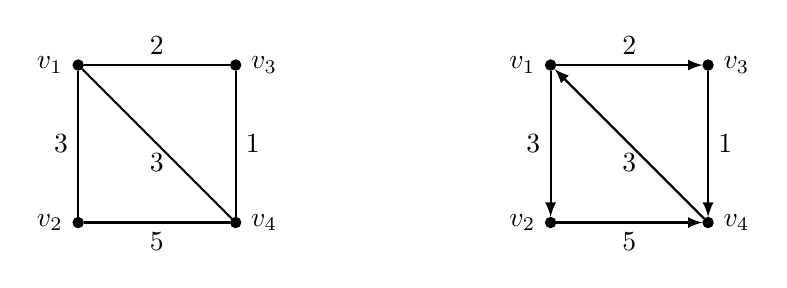
\begin{tikzpicture}
      \tikzset{enclosed/.style={draw, circle, inner sep=0pt, minimum size=.13cm, fill=black}}
%% Vertices
	%ikke orienteret
      	\node[enclosed, label={left, above: $v_1$}] (v1) at (0,2) {};
     	\node[enclosed, label={left, below: $v_2$}] (v2) at (0,0) {};
     	\node[enclosed, label={right, above: $v_3$}] (v3) at (2,2) {};
     	\node[enclosed, label={right, below: $v_4$}] (v4) at (2,0) {};
	%orienterede
		\node[enclosed, label={left, above: $v_1$}] (1v1) at (6,2) {};
     	\node[enclosed, label={left, below: $v_2$}] (1v2) at (6,0) {};
     	\node[enclosed, label={right, above: $v_3$}] (1v3) at (8,2) {};
     	\node[enclosed, label={right, below: $v_4$}] (1v4) at (8,0) {};
%Edges
	%Ikke orientered
		\path [thick] (v1) edge node[midway, left] {3} (v2);
		\path [thick] (v1) edge node[midway, above] {2} (v3);
		\path [thick] (v2) edge node[midway, below] {5} (v4);
		\path [thick] (v3) edge node[midway, right] {1} (v4);
		\path [thick] (v1) edge node[midway, below] {3} (v4);
	%orienterede
		\path [->, > = latex, thick] (1v1) edge node[midway, left] {3} (1v2);
		\path [->, > = latex, thick] (1v1) edge node[midway, above] {2} (1v3);
		\path [->, > = latex, thick] (1v2) edge node[midway, below] {5} (1v4);
		\path [->, > = latex, thick] (1v3) edge node[midway, right] {1} (1v4);
		\path [->, > = latex, thick] (1v4) edge node[midway, below] {3} (1v1);

	\end{tikzpicture}
	\caption{Ikke-orienteret, vægtet graf (venstre) og orienteret, vægtet graf (højre).}
	\label{fig.vaegteteks}
\end{figure}